%===================================== CHAP 4 =================================

\chapter{Methods}

Now we move to the context of neurons and synapses. In section \ref{set_up} the different elements included in the model are introduced and the most important equations from GLM and MCMC are defined for this system. Simulated experiments with two neurons and one directed synaptic connection was performed for test purposes. Various approaches for inferring time varying weighs were tried and their limitations were investigated. In section \ref{Method} the methods of the test experiments are described in detail. Section \ref{Precalc} presents some calculations based on probability theory to say something about how well the method is expected to perform.

\section{Model}
\label{set_up}

\subsection{Framework}
As described in section \ref{Lab}, the data material is the time points for action potentials in time interval $[0,K]$ for the N neurons, as given by equation \ref{eq:AP}. Let the time line be divided into T equally sized bins, and number these bins,

\begin{equation}
    t \in \{1, 2, ..., T\}.
\end{equation}

Also, let $s_{i}(t) \in \{0,1\}$ be a binary variable taking value 1 if neuron $i$ fires at least once in the time bin $t$, and 0 otherwise. This is illustrated in figure \ref{fig:spike_train}, where the top array is a spike train, and the bottom array is the corresponding binary values for the time bins.

\begin{figure}[h]
\caption{Upper time line illustrates the time points, $a_x$, for action potentials. Bottom time line illustrates the corresponding binary value for the defined time bins.}
\label{fig:spike_train}
    \centering
    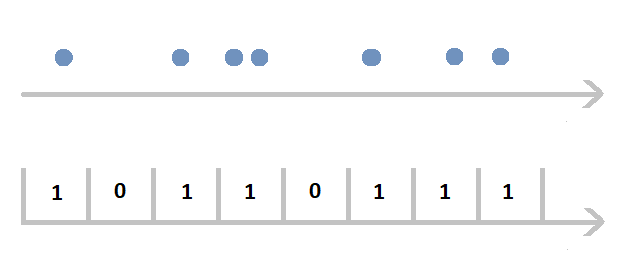
\includegraphics[scale=0.7]{Sp_t.png}
\end{figure} 

The variable $s_{i}(t)$ can be considered a stochastic variable from a Bernoulli process. It has expected value $\lambda (t)$, also referred to as \textit{spike rate}, that can be understood as the probability that the neuron will fire in the time bin $t$. The value of this spike rate is calculated from some linear predictor, $\eta_i(t)$ through a logit link function. 

\begin{equation}
\label{eq:prob}
\begin{split}
P(s_i(t)|\lambda_i(t)) =  Ber(\lambda_i(t)) = \lambda_i(t)^{s_i(t)}(1-\lambda_i(t))^{1-s_i(t)}, \\ \lambda_i(t) = h(\eta_i(t))= \frac{exp(\eta_i(t))}{1+exp(\eta_i(t))}.
\end{split}
\end{equation}

The linear predictor is a linear combination of the states of the neurons at the previous time step and a background noise, $b_i$. This is expressed as,

\begin{equation}
\label{eq:lin_pred}
    \eta_i(t) = \Big (\sum_{j=0}^{N}  w_{ji}(t)s_j(t-1) \Big) + b_i.
\end{equation}

Here $w_{ji}$ is a \textit{weight} between neuron $j$ and neuron $i$, and represents the strength of the connection between the two neurons. The contribution to the linear predictor for $\lambda_i(t)$ from neuron $j$ is $w_{ji}s_j(t-1)$. A positive value for $w_{ji}$ corresponds to an excitatory synaptic connection, whereas a negative weight represents an inhibitory one. A weight with value zero, means that there is no connection. Typically these weights are considered as fixed. However, as the aim is here to study the synaptic plasticity, the weights are let to vary with time. Therefore, we set $w_{ji} = w_{ji}(t)$. The connectivity of the whole network of neurons can be summarized by a time dependent $N \times N$ weight matrix, $W(t)$, which for three neurons would look like, 

\begin{equation*}
W(t) = 
\begin{pmatrix}
w_{11}(t) & w_{12}(t) & w_{13}(t)\\
w_{21}(t) & w_{22}(t) & w_{23}(t)\\
w_{31}(t) & w_{32}(t) & w_{33}(t)\\
\end{pmatrix}.
\end{equation*}

The weights are unknown, and are the parameters that we want to infer from the spike data. 


%For the whole system of neurons, the probability for the state at time $t$ is,

%\begin{equation}
    %P(S_t|W_t) = \prod_{i,t} P(s_{it}|S_{t-1}, W_t).
%\end{equation}

 %where $\{t_1, t_2, ..., t_n\}$ is \ a sequence of equally spaced time steps in [0,T], where $t_{k}-t_{k-1} = t_1$.  To keep as much information as possible, it is preferable to set the time intervals so small that there is very low probability that the neuron will spike more than once in the intervals. Then, at time $t$ we have a collection of $N$ sequences

%\begin{equation}
    %S_{t} = \{\{s_{i,t_1}, ,...,s_{i,t-1},s_{it}\}\}_{i=0}^{N} \quad s_{i,t_k} \in {0,1}
%\end{equation}


\subsection{Inferring time varying weights}
The goal is to infer the time varying weighs given the set of spiking values. As mentioned in chapter \ref{ch:theory} it is preferable to use a Bayesian approach, so one can include prior information. The prior will later be defined in terms of learning rules, but for this project it is set to be a restriction on how much a weight is allowed to vary from one time step to another. So, the prior distribution to be used is a gaussian distribution for each $w_{ji}(t)$ centered at $w_{ji}(t-1)$, each with standard deviation $\sigma$, namely

\begin{equation}
    P(W) = \frac{\exp(-\Gamma /2\sigma)}{\sqrt{2\pi \sigma}},
\end{equation}

where $W=\{W(t)\}_{t=1}^N$, and

\begin{equation}
    \Gamma = \sum_{j=0}^{N} \sum_{t=0}^{T-1} (w_{ji}(t+1)-w_{ji}(t))^2.
\end{equation}

Even though this is a simple prior to be used to test purposes, it is reasonable since we know that the true weights are correlated in time. 

Let $S(t) = \{s_i(t)\}_{i=1}^N$ be the collection of spike data for all the neurons at time $t$. As deduced from equation \ref{eq:prob} and \ref{eq:lin_pred}, all information about the spike rate of neuron $i$, $\lambda_i(t)$, is covered by the weights, the spike data in time step $t-1$ and the background rate $b_i$. Since the spike data and the background rate is considered as know, we can set

\begin{equation}
    P(s_i(t)|\lambda_i(t)) = P(s_i(t)|S(t-1),W(t), b_i) = P(s_i(t)|W(t)),
\end{equation}

which is the likelihood of $s_i(t)$ given some specified $W(t)$. The likelihood for all the spike data, $D=\{S(1), S(2)...,S(T)\}$ is then

\begin{equation}
    P(D|W) = \prod_{i,t} P(s_i(t)|W(t)).
\end{equation}

Hence, we have the following expression for the posterior distribution for the weights

\begin{equation}
\label{Posterior}
        P(W|D) = \frac{P(D|W)\times P(W)}{P(D)} = \frac{\Big\{\prod_{i,t} P(s_{i}(t)|S(t-1), W(t))\Big\} \times \Big\{\frac{\exp(-\Gamma /2\sigma)}{\sqrt{2\pi \sigma}}\Big\}}{P(D)}, 
\end{equation}

where

\begin{equation}
        P(D) = \int \Big\{\prod_{i,t} P(s_{i}(t)|S(t), W(t))\Big\} \times \Big\{\frac{\exp(-\Gamma /2\sigma)}{\sqrt{2\pi \sigma}}\Big\} d{W}.
\end{equation}

Since Metropolis-Hastings will be used for making inference, there is no need to compute the denominator, $P(D)$. The value that is necessary to compute is the ratio between the posterior distribution for some suggested weights $W'$ and for some "current" weights $W$. The product of factors less then one will decrease towards zero as the number of factors increases. Therefore, to avoid computer rounding to zero of the likelihood for a large number of time steps, it is necessary to use the log values for computations instead. The relevant value to compute in each iterations is the following,

\begin{equation}
\label{eq:ratio}
\begin{split}
    \log \frac{\big \{ \prod_{i,t} P(s_{i}(t)|S(t-1), W(t)'\big \} \times \exp(-\Gamma' /2\sigma)}{\big \{ \prod_{i,t}  P(s_{i}(t)|S(t), W(t)) \big \} \times \exp(-\Gamma /2\sigma)} \\
    = \Big \{ \sum_{i,t} \log( P(s_{i}(t)|S(t-1), W(t)')) - \log( P(s_{i}(t)|S(t-1), W(t)) \Big \} -\Gamma' /2\sigma +  \Gamma /2\sigma
\end{split}
\end{equation}

The parameters, $\sigma$, will be referred to at the \textit{prior standard deviation}. This can be adjusted to vary the dominance of the prior distribution. 


\section{Method for test cases}
\label{Method}

In this project three test cases was performed on a simple system consisting of two neurons, 1 and 2, and a synaptic weight, $w_{12}$ directed from neuron 1 to neuron 2.

\begin{figure}[h]
    \centering
    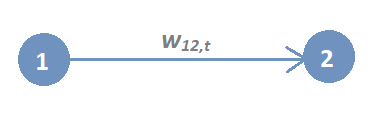
\includegraphics[scale=0.6]{Two_neurons_illustration.png}
\end{figure}

Neuron 1 has a constant probability for spiking, according to a background parameter $b_1$. Neuron 2 has spiking probability that depends on the spiking of $N_1$ in the previous time step through the linear predictor $b_2 + w_{21}(t) \cdot s_{1}(t-1)$. The actual spiking rate is related to the linear predictor through a logit link, as described in section \ref{sec:Bernoulli}. The distributions of the stochastic variables $s_{i}(t)$, representing the spiking in this system, are given by equation \ref{Eq:TestCase}.

\begin{equation}
\begin{split}
\label{Eq:TestCase}
    s_{1}(t) \sim \text{Ber}(\pi_{1}(t)) \hspace{3cm} \pi_{1}(t)= \frac{1}{1+e^{-b_1}} \\
    s_{2}(t) \sim \text{Ber}(\pi_{2}(t)) \hspace{1cm} \pi_{2}(t)= \frac{1}{1+e^{-(b_2 + w_{21}(t) \cdot s_{1}(t-1)}}
\end{split}
\end{equation}

Typical parameter values to be used in the test cases are 0.5 and 1 for b1, and -1 and 0 for b2. The value for the weight $w_{12}$ will be let to vary with time, but a typical size for it will be $w_{12}=0.7$. To get a better intuition it is useful to translate this to the corresponding firing rates. Table \ref{table:parameters} shows the resulting firing rates for the different parameter values


\begin{table}[!h]
\centering
\begin{tabular}{|c|c|c|c|}
	\hline
	Neuron & b & \pi_{s_{1}(t-1)=0} & \pi_{s_{1}(t-1)=1} \\
	\hline\hline
	1 & 0 & 0.5 & 0.5\\
	\hline
	1 & 0.5 & 0.62 & 0.62\\
	\hline
	2 & -1  & 0.27 & 0.43\\
	\hline
	2 & 0  & 0.5 & 0.77\\
	\hline
\end{tabular}
\caption{Background parameter and corresponding spiking rates for neuron 1 and neuron 2}
\label{table:parameters}
\end{table}

The purpose of all the test cases was to infer the underlying weights given the spike train data. Normalizes root mean square error (rnMSE) was used measure the goodness of the various test cases. This was calculated according to the following equation,

\begin{equation}
    rnMSE = \sqrt{\frac{\sum_t(w_{12}(t)^I-w_{12}(t))^2}{\sum_t w_{12}(t)^2}},
\end{equation}

where $w_{12}(t)^I$  are the inferred weights and $w_{12}(t)$ are the generative weights.

\subsection{CASE 1: Inferring constant weight with Newton method}
\label{sec:CASE1}

The series of Bernoulli variables $\{s_{1}(t)\}_{t=1}^T$ and $\{s_{2}(t)\}_{t=1}^T$ were drawn according to equations \ref{Eq:TestCase}, with constant weight $w_{21}(t) = w_{21} = 0.7$ and $T=1000$. The score and Fisher value for this situation is 

\begin{equation}
\begin{split}
    score(w_{12}) = \sum_{t=2}^{T} s_{1}(t-1) (s_{2}(t)-\pi_{2}(t)), \\
    H(w_{12}) = \sum_{t=2}^T s_{1}(t-1)^2 \pi(t)(1-\pi(t)) = \sum_{t=1}^T s_{1}(t-1) \pi(t)(1-\pi(t)).
\end{split}
\end{equation}

The last equivalence is valid since $s_{1}(t)$ only can take values 1 or 0. 

An initial guess was set to $w_{12}^{(0)} = 2$. Newton iterations, as given by equation \ref{eq:Newton}, were performed until convergence.\\ 

\subsection{CASE 2: Inferring dynamic weights with Metropolis-Hastings}
\label{sec:CASE2}
Now the weights were let to vary, and the aim was to infer the vector ${\bf w_{12}}$ of length T, of weights for each time step. In this test case 10 time steps was used, $T=10$. In the first time step, there is no "previous step" that can be used to evaluate the spike rate of neuron 2. Therefore, in this time step the only thing happening is generating the variable $s_{1}(1)$. This means that there are 9 weights to infer, corresponding to $t=2,...,10$. From $t=2$, spikes for both neurons are generated, where the spike rate for neuron 2 is computed according to value of the linear predictor. 

Before simulating spiking of the two neurons, the generative weight trajectory was specified. The weight at $t=2$ was set to 0.7, and the remaining weights were drawn as

\begin{equation}
    w(t) = w(t) + |n(0,0.001)|,
\end{equation}

where $|n(0,0.001)|$ is the absolute value of a normal distributed parameter with zero mean and variance equal to $0.001$. The absolute value is used so that the weight trajectory imitates a connection that strengthens over time. Figure \ref{fig:Generative} shows an example of how a typical generative weight trajectory for this test case looks like. 

\begin{figure}
\caption{Example generative weight trajectory in case 2}
\label{fig:Generative}
    \centering
    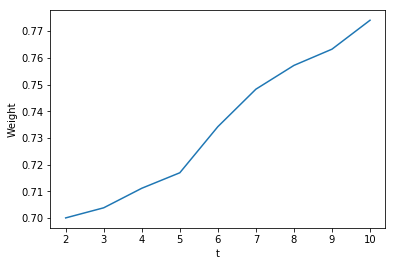
\includegraphics[scale=0.8]{fig/UL.png}
\end{figure}


In reality the number of time steps is much larger, and changing much slower. However, few time steps is used in this test case for simplicity and shorter running time. Therefore, the plasticity is set high so that it is possible to investigate whether the algorithm can infer time varying weights and not only approximates to a constant value. 

Spike trains for the two neurons were again drawn according to equation \ref{Eq:TestCase}, this time using the generated time varying weights. These spike trains were drawn various number of times for the same weight trajectory, for comparing the goodness of the algorithm for different amounts of data. In other words, for one weight trajectory $\{w_{12,t}\}_{t=1}^T$ it was simulated spike trains
$\{\{s_{1}(t)_i\}_{t=1}^T\}_{i=1}^I$ and $\{\{s_{2}(t)_i\}_{t=1}^T\}_{i=1}^I$ with $I \in \{1,10,100,1000,10000 \}$.

To infer the weights from the data, the Metropolis-Hastings algorithm was used. In the algorithm the expression given by \ref{eq:ratio} needs to be computed in every iteration. For this two neuron system, these equations are calculated as

\begin{equation}
\begin{split}
    l({\bf w_{12}}) = \sum_i \sum_t s_{2,i}(t)(b_2 + w_{12}(t)*s_{1,i}(t-1)) - log(1 + exp(b_2 + w_{12}(t) * s_{1,i}(t-1))) \\
    \Gamma({\bf w_{12}}) = \sum_{t=2}^T (w_{12}(t) - w_ {12}(t-1))^2\\
    \log ( \alpha) = l({\bf w_{12}}') - l({\bf w_{12}}) - \Gamma({\bf w_{12}}')/2\sigma + \Gamma({\bf w_{12}})/2\sigma.
\end{split}
\end{equation}

In this case the prior variance was equal to $ 0.0001$. The proposal distribution used was a multivariate normal distribution with mean vector equal to the weight trajectory from the last iteration, variances equal to $0.0001$ and zero covariances. 
The Metropolis-Hastings procedure for this case is summarized in algorithm \ref{alg:M-H}.

\begin{algorithm}
\caption{}\label{alg:M-H}
\begin{algorithmic}
\State Create empty list $[]$ for weight sample
\State Set start guess ${\bf w_{12}} = {\bf w_{12}}^{(guess)}$
\For {$iteration=1,2,\ldots$}
\State Draw ${\bf w_{12}}'$ from proposal distribution
\State Compute $log(\alpha)$
\State Compute $\alpha = exp(log(\alpha))$
\If {$\alpha > 1$}
\State ${\bf w_{12}} = {\bf w_{12}}'$
\Else 
\If {random.uniform(0,1) $<\alpha$}
\State ${\bf w_{12}} = {\bf w_{12}}'$
\EndIf
\EndIf
\State Add ${\bf w_{12}}$ to sample list
\EndFor
\end{algorithmic}
\end{algorithm}

Two variants of this procedure was performed. First, the initial guess was set equal to the generative weights. This gives insight into how well the procedure manages to stay at the correct solution. In reality the true weights are not known. Therefore, it is also relevant to check whether the generative weights can be inferred when starting somewhere else. So in the second variant the initial guess was a random walk around 1. 

\subsection{CASE 3: Weights generated by learning rule}
In reality it is not possible to perform multiple spiking replicates for the same weight trajectory. If the synaptic connections are changing according to learning rules, as presented in section \ref{sec:LR}, the weight updates are dependent on the spiking as time goes by. Since the spiking is a random process, it cannot be reproduced properly. Therefore, we have to rely on only one spike train per neuron, for one weight trajectory. However, in reality the time series is longer and the weights are changing slower and are strongly correlated in time. 

So in this test case weights and the spikes were generated simultaneously, by means of the STDP learning rule, given by equation \ref{eq:STDP}. The parameter values used for the learning rule were the same as the ones suggested in \cite{Song}, namely $\tau_{\pm} = 20 ms$, $A_+ = 0.005$ and $A_- = 1.05 \times A_+$. The learning rule with these parameters is illustrated in figure \ref{fig:LR}.

\begin{figure}[hbt!]
\caption{STDP learning rule}
\label{fig:LR}
    \centering
    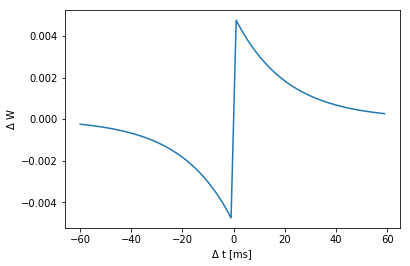
\includegraphics[scale=0.8]{fig/Learning_rule2.png}
\end{figure}

This time $T$ and the spiking rates was set to illustrate realistic time relations. In \cite{Linderman} they use a baseline firing rate with mean 20Hz. To roughly have the same firing level the model was set to have 40 time stamps for representing one second, and the firing rate of the two neurons around one half. 

First the procedure in algorithm \ref{alg:M-H} was performed with 10 seconds (400 time stamps). The weight trajectory drawn for this is plotted in figure \ref{fig:w_STDP}. 


\begin{figure}[hbt!]
\caption{Generative weights drawn according to the STDP rule and the generated spikes}
\label{fig:w_STDP}
    \centering
    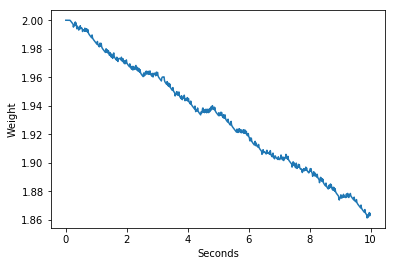
\includegraphics[scale=0.8]{fig/LR_underllying.png}
\end{figure}

An easy way to simplify the problem and to utilize the time correlations is to specify equally sized time windows and assume that the weight is constant within each window. Since we have restricted the degrees of freedom this can only give a rough estimate of the weights. However, this can still be useful to investigate whether we can characterize the learning trends with only one spike trajectory. The learning rule itself has much fewer parameters than the number of weights. 



\section{Precalculations}
\label{Precalc}

\begin{itemize}
    \item The aim here is to calculate how well I expect my tests to work. Can use hypothesis testing on bernoulli GLM 
    \item Say something about how many time points ect that is needed to be able to detect a change of the weights
\end{itemize}

\begin{wraptable}{r}{4cm}
\begin{center}
 \begin{tabular}{||c c c ||} 
 \hline
 n & Lower & Upper \\ [0.5ex] 
 \hline\hline
 10 & 0.5 & 1 \\ 
 \hline
 100 & 0.7 & 0.84 \\
 \hline
 1000 & 0.748 & 0.792 \\
 \hline
 10000 & 0.7631 & 0.7769 \\ [1ex] 
 \hline
\end{tabular}
\end{center}
\end{wraptable}

\begin{figure}[h]
    \centering
    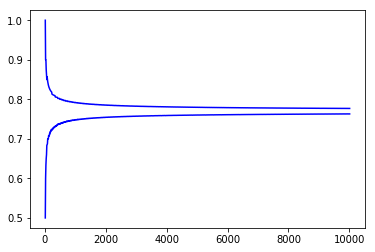
\includegraphics[scale=0.7]{Conf_intervals.png}
\end{figure}

It is practical to have some understanding of how precisely the weights can be inferred from the spike data. When performing $n$ repeated trials of a Bernoulli process with success rate $\pi$, the sum successes comes from a binomial distribution, with parameters $n$ and $\pi$. For some success count, $n_{success}$, the parameter $\pi$ can be estimated as $\frac{n_{success}}{n}$. How good this estimate is depends on the number of trials, $n$. Figure ?? and table ?? presents the endpoints of range that contains 90\% of the distribution, for different values of n (scaled by one over n). 